\section{Testing \& Evaluation}
\label{sec:test}

No single tool certifies accessibility: automated checkers catch only a fraction of real barriers
(W3C's own position), so the rest needs human judgement and task evidence. We therefore
\textbf{triangulate} across four layers (Figure~\ref{fig:layers}) and --- just as important ---
separate \emph{raw suggestions} from \emph{confirmed defects}.

\begin{figure}[h]
\centering
\begin{tikzpicture}[
  l/.style={rounded corners=4pt,draw,line width=0.8pt,minimum height=0.85cm,align=center,font=\small,text width=12.5cm,fill=softbg},
  e/.style={-{Stealth[length=2mm]},draw=slate}
]
  \node[l,draw=brandblue] (a) {\textbf{1. Static / semantic} --- Layout Inspector, review the Semantics Tree};
  \node[l,draw=brandblue,below=3mm of a] (b) {\textbf{2. Automated interaction} --- Compose UI Testing + ATF on fixed states};
  \node[l,draw=brandblue,below=3mm of b] (c) {\textbf{3. Assistive technology} --- TalkBack across the end-to-end flow};
  \node[l,draw=brandgreen,below=3mm of c] (d) {\textbf{4. User evaluation} --- observe users with access needs (when possible)};
  \draw[e] (a)--(b); \draw[e] (b)--(c); \draw[e] (c)--(d);
\end{tikzpicture}
\caption{The layered evaluation model. Each layer answers a different question; no single layer is
sufficient on its own.}
\label{fig:layers}
\end{figure}

\subsection{Manual testing with TalkBack}

TalkBack is the ground truth for the listening experience. Our protocol runs each core flow twice:
first swiping linearly to check focus order and labels, then exploring by touch to compare the visual
region with the focus region. For every important control we activate it and verify the role, state,
and \emph{post-action focus}. Common issues this surfaces --- and which pure automation misses ---
are wrong or missing labels, focus that jumps after a dialog, over-merged cards that hide a child
action, and dynamic changes (buffering, errors) that are never announced. We record each finding with
a severity, reproduction steps, and expected-vs-actual behaviour.

\subsection{Accessibility Scanner --- and an honest case study}

Accessibility Scanner evaluates a screen on-device and draws orange boxes around potential issues
(labels, touch targets, contrast). To practise the \emph{evidence-collection workflow} --- not to
judge another company's app --- we captured a 15-screen flow through Agoda
(Figure~\ref{fig:scanner}). The point of the exercise is methodological: how to record, de-duplicate,
and interpret tool output responsibly.

\begin{figure}[h]
\centering
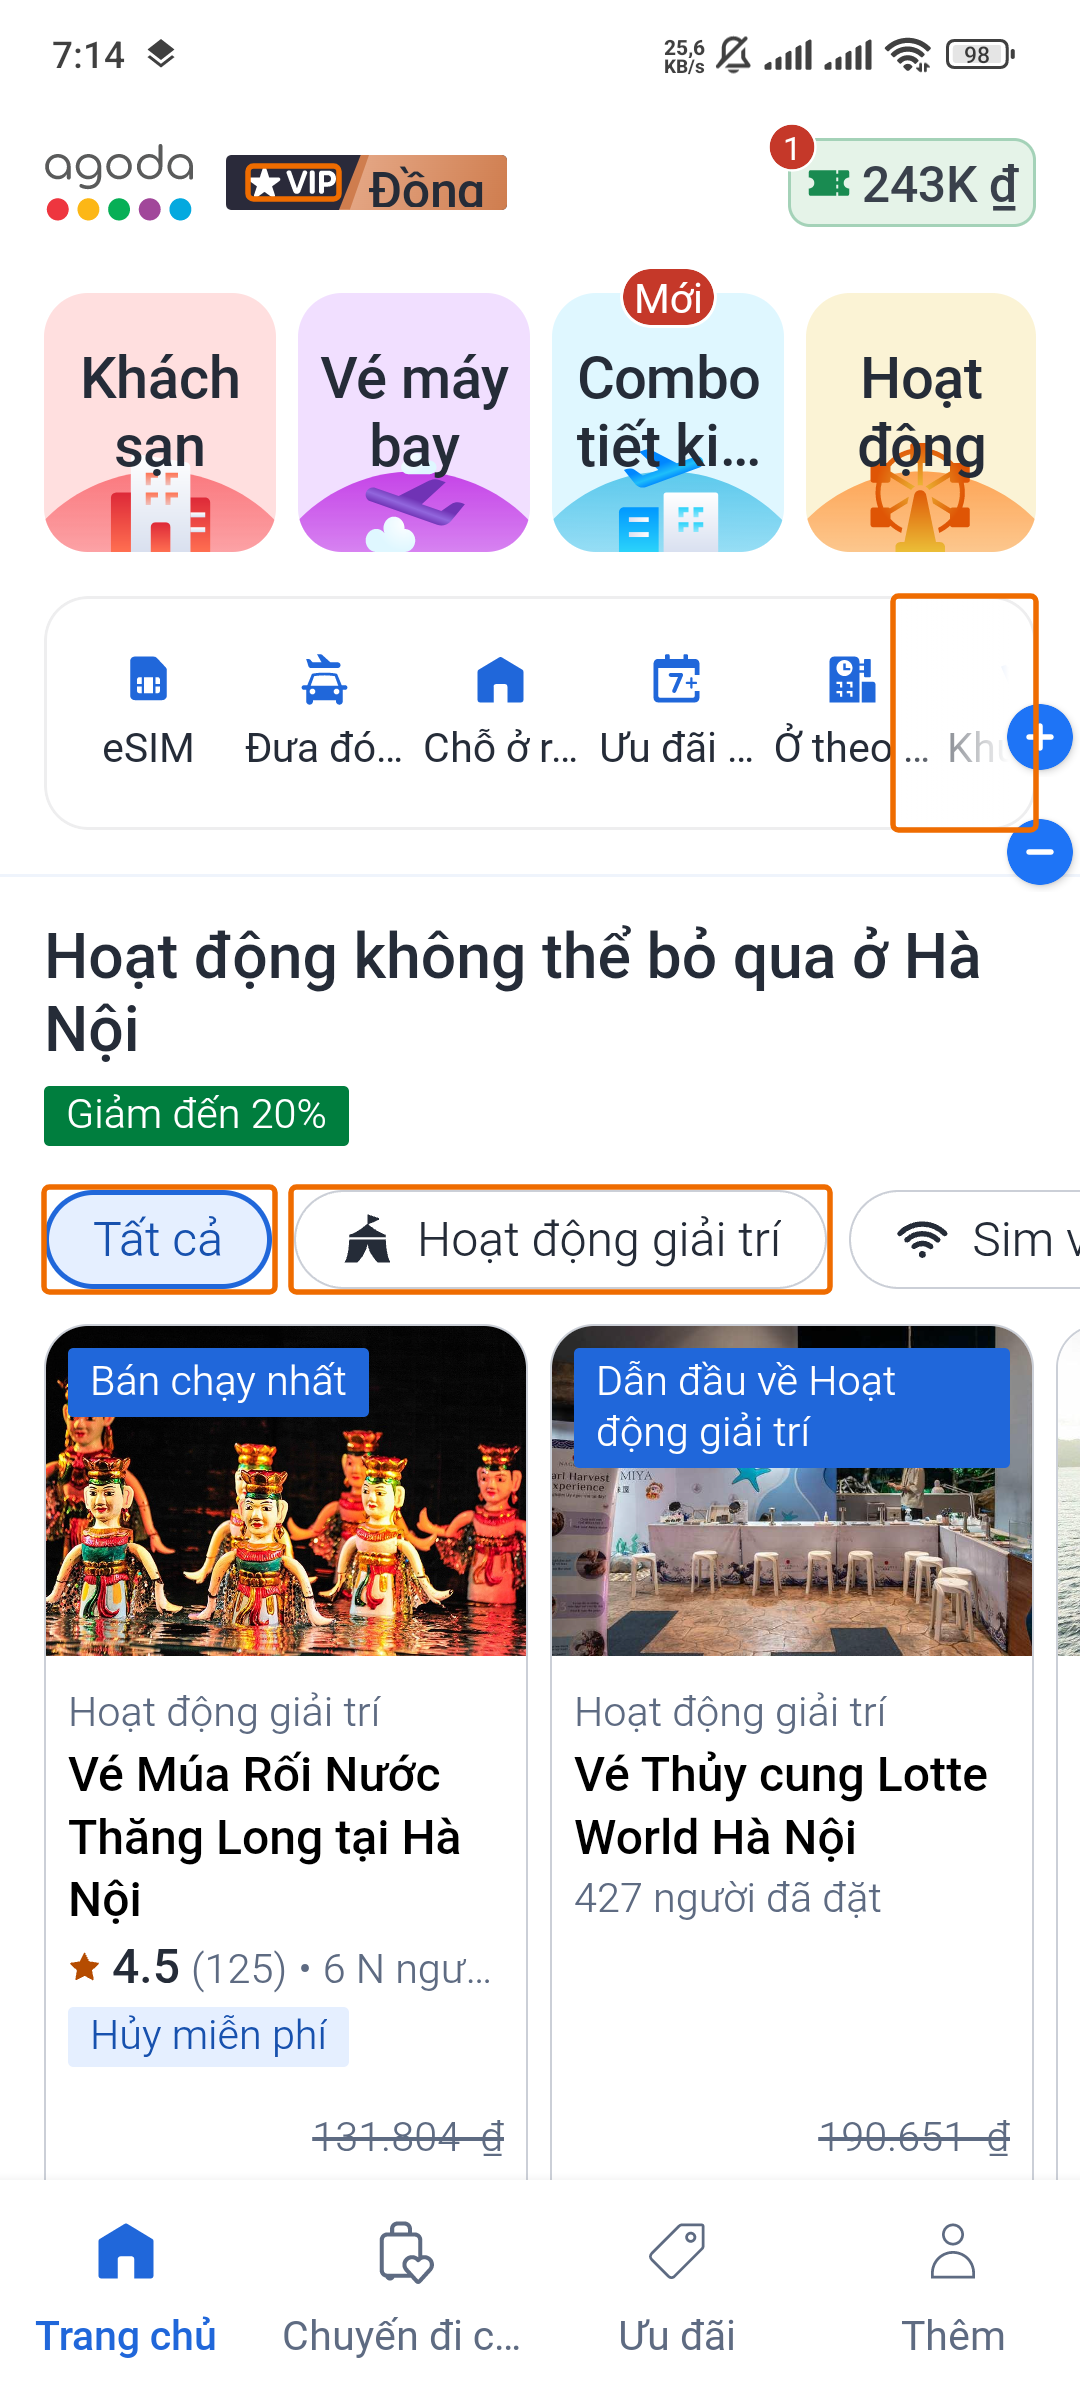
\includegraphics[height=8.6cm]{images/scanner_agoda.png}
\caption{Accessibility Scanner on a real app (Agoda), used only to rehearse the workflow. Orange
boxes mark raw \emph{suggestions} --- e.g. a 38\,dp touch target below the 48\,dp guideline and chips
that may lack a distinct label. Raw suggestions are not confirmed defects.}
\label{fig:scanner}
\end{figure}

The 15-screen capture produced \textbf{102 raw suggestions}, distributed as in
Figure~\ref{fig:dist}. These numbers must be read carefully: they are \emph{not} 102 independent,
confirmed bugs. Loading/skeleton states, web-view content, and the \emph{same} chip appearing across
several frames all inflate the count (report~2 and report~14 overlap; the splash screen produced
none). The correct next step is de-duplication by root cause and confirmation with TalkBack ---
never turning a warning into a conclusion without reproducing it.

\begin{figure}[h]
\centering
\begin{tikzpicture}
  \def\barh{0.55}
  % axis
  \draw[slate] (0,0) -- (10.5,0);
  \foreach \x/\lbl in {0/0,2/10,4/20,6/30,8/40,10/50} {
    \draw[slate] (\x,0)--(\x,-0.1) node[below,font=\scriptsize]{\lbl};
  }
  % bars: value scaled x/5
  \foreach \i/\val/\name/\col in {0/55/{Touch target (53.9\%)}/brandblue, 1/25/{Item label (24.5\%)}/brandgreen, 2/20/{Text contrast (19.6\%)}/codeann, 3/2/{Duplicate desc. (2.0\%)}/warnred} {
    \fill[\col] (0,{1.4+\i*(\barh+0.55)}) rectangle ({\val/5},{1.4+\i*(\barh+0.55)+\barh});
    \node[right,font=\scriptsize] at ({\val/5+0.15},{1.4+\i*(\barh+0.55)+\barh/2}) {\name --- \val};
  }
  \node[font=\scriptsize\color{slate}] at (5,-0.55) {number of raw suggestions};
\end{tikzpicture}
\caption{Distribution of the 102 raw suggestions across the 15-screen Agoda capture. Touch-target
warnings dominate, but this is a \emph{starting hypothesis}, not a root-cause finding.}
\label{fig:dist}
\end{figure}

\subsection{Layout Inspector, Compose UI Testing, and ATF}

Once we have our own source, three developer tools close the loop:

\begin{itemize}[leftmargin=1.4em]
  \item \textbf{Layout Inspector} shows the live merged and unmerged semantics trees, linking a
        TalkBack/Scanner symptom to a specific node --- a diagnostic tool, not a verdict on user
        experience.
  \item \textbf{Compose UI Testing} asserts semantics contracts in CI: that a control has the
        accessible name a screen reader will speak, and \code{printToLog()} dumps the tree for
        diagnosis. Our \code{AccessibilityTest.kt} does exactly this.
  \item \textbf{Accessibility Test Framework (ATF)}, Google's open-source rule engine, adds
        automated checks for speakable text, touch-target size, and contrast, usable as a CI quality
        gate.
\end{itemize}

\begin{lstlisting}[caption={\texttt{AccessibilityTest.kt} --- assert a spoken name, then dump the tree.},captionpos=b]
// 1. The icon-only search button must expose a spoken label, not just a glyph.
composeRule.onNodeWithContentDescription("Search podcasts").assertExists()

// 2. Dump the unmerged tree to verify merge/clear behaviour on the cards.
composeRule.onRoot(useUnmergedTree = true).printToLog("A11Y_TREE")
\end{lstlisting}

Table~\ref{tab:tools} positions each tool against the others.

\begin{table}[h]
\centering
\small
\begin{tabularx}{\textwidth}{@{}l l l Y@{}}
\toprule
\textbf{Tool} & \textbf{Source?} & \textbf{Mode} & \textbf{Best for / cannot replace} \\
\midrule
TalkBack & No & Manual & Listening experience, focus, end-to-end flow. \\
Accessibility Scanner & No & Semi-auto & Fast visual triage of labels/targets/contrast; not coverage. \\
Layout Inspector & Debug build & Manual & Inspect merged/unmerged tree; not user experience. \\
Compose UI Testing & Yes & Automated & Semantics contracts \& regression; not utterance quality. \\
ATF & Yes & Automated & Standardised checks in CI; not real usability. \\
\bottomrule
\end{tabularx}
\caption{Complementary roles of the five verification tools.}
\label{tab:tools}
\end{table}

\subsection{Evaluation metrics and trade-offs}

A credible evaluation states scope, representative flows, device, versions, and completion criteria,
then reports both automated and task-based measures: first-flow coverage, task-completion rate,
completion time, number of TalkBack gestures, automated pass rate, and a \emph{confirmed-defect
rate} that distinguishes real bugs from raw suggestions. Findings are triaged by \textbf{impact on
the task} --- \emph{Blocker} (task impossible, fix before ship) $>$ \emph{Major} $>$ \emph{Moderate}
$>$ \emph{Minor} --- not merely by count. A missing label on the checkout button outweighs many
touch-target warnings on secondary content.

Every technique in this report is a trade-off, and naming them is part of an honest evaluation:

\begin{itemize}[leftmargin=1.4em]
  \item \code{mergeDescendants} cuts swipes but can hide an independent child action or produce an
        over-long sentence --- measure gesture count \emph{and} listen to the whole utterance.
  \item Rich labels aid comprehension but, if they duplicate role/state, add listening time.
  \item \code{traversalIndex} fixes reading order but hand-tuned indices are brittle and can drift
        from the visual layout; use the minimum number and document why.
  \item Custom controls give design freedom but must re-declare role, state, and keyboard behaviour
        that Material would have provided for free.
\end{itemize}
